\documentclass[conference]{IEEEtran}
\IEEEoverridecommandlockouts
\usepackage{cite}
\usepackage{amsmath,amssymb,amsfonts}
\usepackage{algorithmic}
\usepackage{graphicx}
\graphicspath{{../figures/}}
\usepackage{textcomp}
\usepackage{xcolor}
\usepackage{booktabs}
\usepackage{multirow}
\usepackage{array}
\usepackage{url}
\def\BibTeX{{\rm B\kern-.05em{\sc i\kern-.025em b}\kern-.08em
    T\kern-.1667em\lower.7ex\hbox{E}\kern-.125emX}}

\begin{document}

\title{Out-of-Sample Evaluation of Shock-Augmented\\ Bayesian Vector Autoregressions:\\ A G7 Macroeconomic Study}

\author{\IEEEauthorblockN{Nicholas Hong}
\IEEEauthorblockA{School of Electrical and Electronic Engineering\\
Nanyang Technological University, Singapore\\
nhong001@e.ntu.edu.sg}}

\maketitle

\begin{abstract}
Bayesian vector autoregressions (BVARs) augmented with constructed exogenous
shocks are widely used for macroeconomic forecasting, yet empirical practice
frequently omits the safeguards needed to interpret their results. Using five
quarterly U.S.\ series over 2000--2025, we assemble a reproducible pipeline that
exposes and corrects several common failures. We show that a na\"ively coded
Minnesota prior can leave the posterior effectively unshrunk, yielding an
explosive companion matrix (largest eigenvalue $1.068$); a natural-conjugate
Minnesota prior implemented through dummy observations restores stability
($0.96$) and bounded forecasts. We document that stacking all available shocks
inflates out-of-sample error by an order of magnitude relative to a no-shock
baseline, that look-ahead leakage in standardized shock construction flatters
apparent skill, and that a static $13$-quarter evaluation window has no power to
discriminate models. Replacing it with an expanding-window evaluation
($48$ origins) scored by proper density rules (continuous ranked probability
score, log score) and Diebold--Mariano tests shows that a stochastic-volatility
BVAR produces sharper, better-calibrated predictive densities than random-walk
and AR(1) benchmarks for output growth and inflation, with the long-rate block
remaining hard to beat. Johansen testing returns full cointegration rank,
formally justifying estimation in levels, and a diagnostic shows the COVID-19
variance spike is concentrated in output, motivating a variable-specific
stochastic-volatility treatment that recovers both the Global Financial Crisis
and pandemic episodes. Extending the evaluation to a five-economy G7 panel with a
common global oil shock, multiple horizons, and an expanded benchmark set sharpens
these conclusions: Bayesian shrinkage dominates an unrestricted VAR in every
country and is the only feature a Model Confidence Set retains for most variables;
the BVAR significantly outperforms the random walk for output growth and the
policy rate once loss differentials are pooled across countries; and the
constructed shocks improve in-sample fit but not multi-step forecasts. The study
offers a transparent, reproducible evaluation protocol and a cautionary,
cross-country account of where shock-augmented BVARs do and do not add value.
\end{abstract}

\begin{IEEEkeywords}
Bayesian vector autoregression, macroeconomic forecasting, Minnesota prior,
stochastic volatility, density forecast evaluation, local projections,
cointegration.
\end{IEEEkeywords}

\section{Introduction}
Vector autoregressions (VARs) have been a workhorse of empirical
macroeconomics since \cite{sims1980}. Because unrestricted VARs are heavily
over-parameterized, Bayesian shrinkage through the Minnesota prior
\cite{litterman1986,doan1984} has become standard, and large BVARs are now
routinely estimated for forecasting and structural analysis
\cite{bgr2010,koop2010}. A common extension augments the endogenous block with
\emph{exogenous shocks}---series constructed outside the model (oil-price
surprises, credit or fiscal impulses, monetary surprises) and entered as
additional regressors or used to identify structural responses.

While the modeling toolkit is mature, applied work frequently couples it with an
evaluation that cannot support the conclusions drawn. Three failures recur.
First, the Minnesota prior is parameterized through precision/variance
conventions that are easy to invert, so that the intended shrinkage is not
actually imposed. Second, models are compared only against one another, without
the na\"ive benchmarks that define a forecasting ``horse race,'' and without
tests of whether accuracy differences are statistically meaningful---an acute
problem given the short post-2020 evaluation windows now common. Third, shocks
are standardized using full-sample moments, leaking future information into the
out-of-sample period.

This paper assembles a transparent, reproducible pipeline that exposes and
corrects these failures on a concrete dataset---five quarterly U.S.\
macroeconomic series, 2000--2025, with six constructed shocks---and reports
what survives rigorous evaluation. Our contributions are:
\begin{itemize}
\item We give a drop-in natural-conjugate Minnesota BVAR via dummy observations
\cite{bgr2010,sims1998} that, on real data, converts an explosive
ordinary-least-squares (OLS) VAR (largest companion eigenvalue $1.068$) into a
stable posterior ($0.96$) with bounded forecasts.
\item We quantify \emph{shock-combination overfitting}: stacking all six shocks
raises out-of-sample root-mean-squared error (RMSE) by up to $8\times$ relative
to a no-shock baseline, whereas the single most useful shock (oil) yields only
modest gains.
\item We implement an evaluation protocol with random-walk and AR(1) benchmarks,
Diebold--Mariano (DM) tests with the Harvey--Leybourne--Newbold (HLN)
small-sample correction \cite{dm1995,hln1997}, and proper density scores
\cite{gneiting2007}, and show that an expanding-window design recovers the
statistical power that a $13$-quarter window lacks.
\item We measure the effect of look-ahead leakage in shock construction, showing
that the only statistically significant benchmark improvement disappears once
shocks are built in real time.
\item We use Johansen cointegration testing to justify levels estimation, and a
volatility diagnostic to show that the pandemic variance spike is
output-specific, motivating a variable-specific stochastic-volatility (SV) model
estimated with the Kim--Shephard--Chib (KSC) mixture sampler
\cite{primiceri2005,ksc1998}.
\item We \emph{generalize} the headline forecasting findings to a five-economy
G7 panel (United States, United Kingdom, Canada, Germany, Japan) with a common
globally identified oil shock, horizons $h\in\{1,2,4,8\}$, and an expanded
benchmark set; pooling across countries and applying a Hansen Model Confidence
Set \cite{hansen2011} establishes which conclusions are systematic rather than
U.S.-specific.
\end{itemize}

The empirical bottom line is deliberately measured: once correctly specified and
honestly evaluated, the BVAR's density forecasts beat na\"ive benchmarks for
output growth and inflation, but the gains are concentrated, modest, and---in a
short window---rarely significant; interest-rate variables are barely
distinguishable from a no-change forecast.

\section{Data}
We use quarterly U.S.\ data from 2000Q1 to 2025Q1 ($T=101$). The endogenous
block $y_t\in\mathbb{R}^5$ comprises real GDP growth (year-over-year), CPI
inflation (year-over-year), the real effective exchange rate (REER, year-over-year),
the 10-year Treasury yield, and a short-term policy rate. Six exogenous shocks
are constructed from auxiliary series: West Texas Intermediate crude oil, an S\&P
100 equity-wealth index, personal consumption expenditure, private fixed
investment, nonfinancial-sector debt (a credit impulse), and the cyclically
adjusted primary balance (a fiscal impulse). Table~\ref{tab:vars} summarizes the
variables.

\begin{table}[t]
\caption{Variables.}
\label{tab:vars}
\centering
\footnotesize
\begin{tabular}{@{}lll@{}}
\toprule
Block & Variable & Transformation \\
\midrule
\multirow{5}{*}{Endogenous}
 & GDP growth & YoY \% \\
 & Inflation (CPI) & YoY \% \\
 & REER & YoY \% \\
 & 10y Treasury yield & level \\
 & Policy rate & level \\
\midrule
\multirow{6}{*}{Shocks}
 & Oil (WTI) & AR(1) surprise, $z$-scored \\
 & Equity wealth (S\&P 100) & AR(1) surprise, $z$-scored \\
 & Consumption (PCE) & AR(1) surprise, $z$-scored \\
 & Investment (PFI) & AR(1) surprise, $z$-scored \\
 & Credit impulse & $\Delta$, $z$-scored \\
 & Fiscal impulse (CAPB) & $\Delta$, $z$-scored \\
\bottomrule
\end{tabular}
\end{table}

\section{Methodology}

\subsection{BVAR with a natural-conjugate Minnesota prior}
The reduced-form model with $p$ lags and exogenous regressors $x_t$ (a constant
and the shocks) is
\begin{equation}
y_t = c + \sum_{j=1}^{p} B_j\,y_{t-j} + \Gamma x_t + u_t,
\qquad u_t \sim \mathcal{N}(0,\Sigma).
\end{equation}
Collecting coefficients into $B$ ($k\times n$, $k=np+m$) and stacking
$T$ observations as $Y=XB+U$, the natural-conjugate prior places
$\mathrm{vec}(B)\mid\Sigma \sim \mathcal{N}(\mathrm{vec}(B_0),\,\Sigma\otimes\Omega_0)$
and $\Sigma\sim\mathcal{IW}(S_0,\nu_0)$. The Minnesota specification
\cite{litterman1986} centers each variable's own first lag at $\delta_i$
(unity for persistent levels, below unity for mean-reverting growth rates) and
all other coefficients at zero, with prior variance for the coefficient on lag
$\ell$ of variable $j$ in equation $i$ proportional to
$(\lambda/\ell)^2(\sigma_i/\sigma_j)^2$, where $\sigma_i$ is the residual
standard deviation from a univariate AR($p$) and $\lambda$ controls overall
tightness.

We impose this prior through \emph{dummy observations} \cite{bgr2010,sims1998}.
Artificial rows $(Y_d,X_d)$ are appended so that an OLS regression on the stacked
system $([Y;Y_d],[X;X_d])$ reproduces the conjugate posterior. The blocks encode
(i) the own- and cross-lag prior with harmonic lag decay scaled by $\lambda$ and
$\sigma_j$, (ii) the inverse-Wishart scale, (iii) a finite, scale-tied prior on
the exogenous coefficients (a near-flat exogenous prior allows posterior draws of
shock coefficients to diverge in short windows), and (iv) a sum-of-coefficients
prior, with tightness $\mu$, that damps near-unit-root behavior. The posterior is
$\Sigma\sim\mathcal{IW}(\tilde S,\tilde\nu)$ and
$\mathrm{vec}(B)\mid\Sigma\sim\mathcal{N}(\mathrm{vec}(\tilde B),\Sigma\otimes\tilde\Omega)$
with $\tilde B=(\tilde X'\tilde X)^{-1}\tilde X'\tilde Y$ on the stacked data.
Forecast stability is monitored through the largest eigenvalue of the companion
matrix.

\subsection{Shock construction and look-ahead leakage}
For the four price-type series the shock is the $z$-scored residual of a
univariate AR(1) on quarterly log growth; for credit and fiscal it is the
$z$-scored first difference. Standardizing with full-sample mean and variance,
and fitting the AR(1) on the full sample, leaks post-sample information into the
shocks used during the evaluation period. We therefore construct two leak-free
variants: a \emph{train-frozen} version, in which AR and standardization
parameters are estimated only through 2021Q4 and then applied out of sample, and
a real-time \emph{rolling} version using a trailing five-year window.

\subsection{Identification: recursive SVAR and local projections}
We contrast two identification philosophies with the exogenous-regressor
approach. A recursive (Cholesky) structural VAR orthogonalizes the reduced-form
residuals under an ordering (output, prices, exchange rate, long rate, policy
rate last), yielding structural impulse responses that depend on that ordering.
Local projections \cite{jorda2005} estimate the horizon-$h$ response by
regressing $y_{t+h}$ on the shock and controls; they are robust to VAR
misspecification but require an identified shock, becoming LP-IV when the shock
is used as an instrument \cite{stockwatson2012,mertensravn2013}.

\subsection{Forecast evaluation}
We evaluate one-step-ahead forecasts in an expanding window: at each origin the
model and benchmarks are re-estimated and a predictive distribution for the next
quarter is formed. Benchmarks are a random walk (no-change) and an AR(1).
Point accuracy is summarized by RMSE; equal predictive accuracy is tested by the
DM statistic with the HLN small-sample correction \cite{dm1995,hln1997}. Density
forecasts are scored by the log predictive score and the continuous ranked
probability score (CRPS) \cite{gneiting2007},
\begin{equation}
\mathrm{CRPS}(F,y)=\mathbb{E}_F|X-y|-\tfrac{1}{2}\,\mathbb{E}_F|X-X'|,
\end{equation}
both reported as means over origins (lower is better), together with the
empirical coverage of the $90\%$ predictive interval. The BVAR predictive
density is the posterior predictive ensemble; benchmark densities are Gaussian
with variance estimated on the training window.

\subsection{Stochastic volatility}
To accommodate time-varying residual variance we use a univariate SV model for
the relevant equation,
\begin{equation}
u_t=e^{h_t/2}\varepsilon_t,\quad \varepsilon_t\sim\mathcal{N}(0,1),\quad
h_t=\mu+\phi(h_{t-1}-\mu)+\eta_t,
\end{equation}
with $\eta_t\sim\mathcal{N}(0,\sigma_\eta^2)$. Estimation uses the KSC
seven-component mixture approximation to $\log\varepsilon_t^2$ together with
forward-filtering backward-sampling for the volatility states
\cite{ksc1998,primiceri2005}. We also considered a single \emph{common}
volatility factor \cite{ccm2016}; Section~\ref{sec:vol} explains why it is the
wrong specification here.

\section{Empirical Results}

\subsection{Integration and cointegration}
Augmented Dickey--Fuller and KPSS tests classify GDP growth and the policy rate
as $I(0)$, inflation and the 10-year yield as $I(1)$, and REER growth as
ambiguous (Table~\ref{tab:coint}). The Johansen trace test returns
\emph{full} cointegration rank ($r=5$) for the system, and full rank again
($r=3$) for the \{10y, policy rate, inflation\} subsystem. Full rank means every
linear combination is stationary: the system has no common stochastic trend to
error-correct, a vector error-correction model collapses to a level VAR, and the
explosive OLS eigenvalue is a small-sample estimation artifact rather than a
unit-root pathology. Estimation in levels with Bayesian shrinkage is therefore
appropriate.

\begin{table}[t]
\caption{Integration order and Johansen cointegration.}
\label{tab:coint}
\centering
\footnotesize
\begin{tabular}{@{}lccc@{}}
\toprule
Variable & ADF $p$ & KPSS $p$ & Verdict \\
\midrule
GDP growth      & 0.006 & 0.10 & $I(0)$ \\
Inflation       & 0.968 & 0.05 & $I(1)$ \\
REER growth     & 0.454 & 0.10 & ambiguous \\
10y yield       & 0.114 & 0.01 & $I(1)$ \\
Policy rate     & 0.002 & 0.10 & $I(0)$ \\
\midrule
\multicolumn{4}{@{}l}{Johansen trace: rank $r=5$ of $5$ $\Rightarrow$ system stationary} \\
\bottomrule
\end{tabular}
\end{table}

\subsection{Specification and stability}
On the real data the OLS VAR is explosive: the largest companion eigenvalue is
$1.068$, and an unshrunk (or mis-shrunk) posterior inherits this, with multi-step
forecasts diverging. The dummy-observation Minnesota BVAR with
$\lambda=0.05$ and sum-of-coefficients tightness $\mu=0.3$ brings the largest
eigenvalue to $0.96$, with $78\%$ of posterior draws stable and bounded
forecasts. Tighter priors are required than textbook defaults precisely because
the data are highly persistent.

\subsection{Shock-combination overfitting}
Table~\ref{tab:horse} reports the static one-step RMSE over 2022Q1--2025Q1 for a
no-shock baseline, the single best shock per equation, and all six shocks
together. Stacking all shocks is dramatically worse than using none---GDP RMSE
rises from $0.60$ to $4.59$ and REER from $2.82$ to $8.28$---a textbook
manifestation of over-parameterization on $\sim\!83$ training quarters. The best
single shock helps only modestly, and oil is the most consistently useful,
winning three of five equations. This pattern cautions against the common
instinct to add shocks cumulatively.

\begin{table}[t]
\caption{Shock-specification ``horse race'': static one-step RMSE,
2022Q1--2025Q1.}
\label{tab:horse}
\centering
\footnotesize
\begin{tabular}{@{}lccc@{}}
\toprule
Variable & Baseline & Best single shock & All shocks \\
\midrule
GDP growth   & 0.604 & \textbf{0.561} (credit) & 4.590 \\
Inflation    & 0.276 & \textbf{0.261} (oil)    & 0.691 \\
REER         & 2.821 & \textbf{2.526} (oil)    & 8.277 \\
10y yield    & 0.534 & \textbf{0.342} (oil)    & 1.896 \\
Policy rate  & 0.544 & \textbf{0.270} (inv.)   & 0.490 \\
\bottomrule
\end{tabular}
\end{table}

\subsection{Out-of-sample point and density evaluation}
A static $13$-quarter window cannot discriminate models: with leak-free shocks
no DM test rejects equal accuracy at the $5\%$ level. We therefore evaluate in an
expanding window from 2013Q1 ($48$ origins), re-estimating every model each
quarter and scoring the full predictive density. Table~\ref{tab:dens} reports
RMSE, CRPS, log score, and $90\%$ coverage for the SV-BVAR and the two
benchmarks; Fig.~\ref{fig:crps} visualizes the CRPS comparison.

The BVAR's predictive densities are sharper and better calibrated than the
benchmarks for GDP growth and inflation on both CRPS and log score, and tie or
beat the long rate on log score; coverage lies in $0.85$--$0.92$, close to the
$0.90$ target. With $48$ origins the DM tests acquire power: GDP beats the random
walk at $p=0.068$ and inflation beats AR(1) at $p=0.051$, in contrast to the
complete absence of significance at $n=13$. The interest-rate block remains hard
to beat---unsurprisingly, a persistent rate is well approximated by a no-change
forecast.

\begin{table}[t]
\caption{Expanding-window one-step evaluation, 48 origins (2013Q1--2025Q1).
RMSE and CRPS: lower is better; log score (LS): higher is better;
$\mathrm{Cov}$: $90\%$ interval coverage.}
\label{tab:dens}
\centering
\footnotesize
\setlength{\tabcolsep}{4pt}
\begin{tabular}{@{}llcccc@{}}
\toprule
Variable & Model & RMSE & CRPS & LS & Cov \\
\midrule
\multirow{3}{*}{GDP growth}
 & SV-BVAR & \textbf{1.785} & \textbf{0.685} & \textbf{$-2.78$} & 0.92 \\
 & RW      & 2.532 & 1.068 & $-3.33$ & 0.88 \\
 & AR(1)   & 2.311 & 0.948 & $-3.30$ & 0.90 \\
\midrule
\multirow{3}{*}{Inflation}
 & SV-BVAR & \textbf{0.379} & \textbf{0.183} & \textbf{$-0.49$} & 0.90 \\
 & RW      & 0.407 & 0.201 & $-0.61$ & 0.83 \\
 & AR(1)   & 0.439 & 0.211 & $-0.78$ & 0.85 \\
\midrule
\multirow{3}{*}{REER}
 & SV-BVAR & 4.321 & 2.117 & $-2.69$ & 0.85 \\
 & RW      & 3.465 & 1.996 & $-2.68$ & 0.90 \\
 & AR(1)   & 3.349 & 1.932 & $-2.64$ & 0.94 \\
\midrule
\multirow{3}{*}{10y yield}
 & SV-BVAR & 0.448 & \textbf{0.215} & \textbf{$-0.44$} & 0.88 \\
 & RW      & 0.383 & 0.216 & $-0.50$ & 0.94 \\
 & AR(1)   & 0.386 & 0.217 & $-0.50$ & 0.92 \\
\midrule
\multirow{3}{*}{Policy rate}
 & SV-BVAR & 0.535 & 0.258 & \textbf{$-0.57$} & 0.88 \\
 & RW      & 0.443 & 0.229 & $-0.65$ & 0.92 \\
 & AR(1)   & 0.460 & 0.236 & $-0.68$ & 0.92 \\
\bottomrule
\end{tabular}
\end{table}

\begin{figure}[t]
\centering
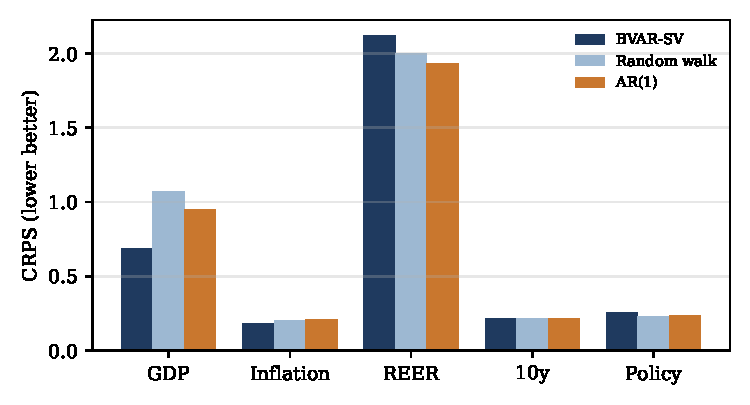
\includegraphics[width=\columnwidth]{fig_crps.pdf}
\caption{Mean CRPS by variable over $48$ expanding-window origins (lower is
better). The SV-BVAR improves on both na\"ive benchmarks for GDP growth and
inflation; the rate variables are close to a no-change forecast.}
\label{fig:crps}
\end{figure}

\subsection{Multiple horizons and an expanded benchmark set}
Table~\ref{tab:horizon} extends the evaluation to horizons $h\in\{1,2,4,8\}$ and
adds two benchmarks that isolate the contribution of each model component: an
unrestricted (OLS) VAR and a no-shock BVAR. Multi-step forecasts are ex ante,
with future shocks set to zero. Two results stand out. First, Bayesian shrinkage
is decisive at every horizon: the unrestricted VAR is far worse than the BVAR
(for GDP, CRPS of $2.27$ versus $1.42$ at $h=4$), confirming that the explosive
OLS dynamics translate into poor forecasts. Second, the constructed shocks do not
help forecasting: the full BVAR and the no-shock BVAR are essentially
indistinguishable across variables and horizons. Because the shocks are observed
only contemporaneously, they aid in-sample fit and identification but cannot
improve genuine multi-step prediction unless the shocks themselves are forecast.
A well-specified AR(1) remains a strong univariate competitor for output.

\begin{table}[t]
\caption{U.S.\ multi-horizon CRPS by model (lower is better). Future shocks set to
zero (ex ante).}
\label{tab:horizon}
\centering
\footnotesize
\setlength{\tabcolsep}{4pt}
\begin{tabular}{@{}llcccc@{}}
\toprule
Variable & Model & $h{=}1$ & $h{=}2$ & $h{=}4$ & $h{=}8$ \\
\midrule
\multirow{5}{*}{GDP growth}
 & BVAR          & 1.048 & 1.158 & 1.418 & 1.227 \\
 & BVAR no-shock & 1.045 & 1.183 & 1.428 & 1.277 \\
 & VAR (OLS)     & 1.493 & 1.863 & 2.266 & 2.104 \\
 & RW            & 1.170 & 1.463 & 1.929 & 1.819 \\
 & AR(1)         & 1.036 & 1.173 & 1.418 & 1.269 \\
\midrule
\multirow{5}{*}{Inflation}
 & BVAR          & 0.210 & 0.346 & 0.589 & 0.830 \\
 & BVAR no-shock & 0.207 & 0.341 & 0.594 & 0.872 \\
 & VAR (OLS)     & 0.302 & 0.509 & 1.013 & 1.093 \\
 & RW            & 0.197 & 0.331 & 0.625 & 1.020 \\
 & AR(1)         & 0.212 & 0.361 & 0.687 & 1.122 \\
\bottomrule
\end{tabular}
\end{table}

\subsection{The cost of look-ahead leakage}
Table~\ref{tab:leak} compares the static one-step RMSE under the (leaky)
full-sample shocks, the train-frozen shocks, and the rolling real-time shocks.
The leakage is modest but systematically flattering: it lowers GDP RMSE
appreciably, and---decisively---the only statistically significant benchmark
improvement under leaky shocks, REER beating the random walk
($p=0.026$), \emph{vanishes} once shocks are built in real time
($p=0.14$ frozen, $p=0.18$ rolling). Apparent skill that does not survive
leak-free construction should not be reported as genuine.

\begin{table}[t]
\caption{Look-ahead leakage: static one-step RMSE by shock construction.}
\label{tab:leak}
\centering
\footnotesize
\begin{tabular}{@{}lccc@{}}
\toprule
Variable & Leaky (full-sample) & Train-frozen & Rolling \\
\midrule
GDP growth  & 0.478 & 0.526 & 0.618 \\
Inflation   & 0.351 & 0.347 & 0.400 \\
REER        & 3.136 & 3.172 & 3.183 \\
10y yield   & 0.467 & 0.475 & 0.481 \\
Policy rate & 0.725 & 0.696 & 0.682 \\
\bottomrule
\end{tabular}
\end{table}

\subsection{Structural responses}
For completeness we report local-projection responses to a one-standard-deviation
oil surprise (Fig.~\ref{fig:lp}). Inflation rises on impact and peaks near
$+0.20$ percentage points after two quarters, and the policy rate climbs steadily
to roughly $+0.37$ after two years---the systematic tightening response to
oil-driven inflation. The early positive output response illustrates that an
unconditional oil-price surprise conflates supply and demand disturbances
\cite{kilian2009}, a caution against treating it as a clean supply shock. A
feasibility check found that, used as instruments in an LP-IV/proxy-SVAR, the
constructed shocks are mostly weak (first-stage $F<10$), with the strongest
apparent instrument (consumption for output) invalid by construction; only oil
provides a defensible, if moderate, instrument.

\begin{figure}[t]
\centering
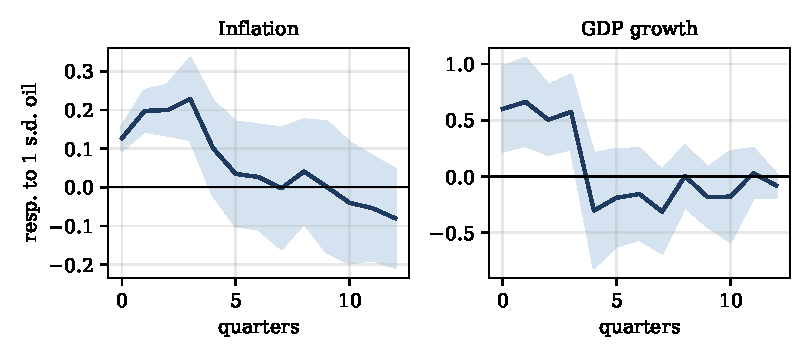
\includegraphics[width=\columnwidth]{fig_lp.pdf}
\caption{Local-projection responses to a one-standard-deviation oil surprise,
with $90\%$ Newey--West bands.}
\label{fig:lp}
\end{figure}

\subsection{Variable-specific volatility}
\label{sec:vol}
The constant-variance assumption fails sharply around 2020: residuals are
$3.9\times$ their normal magnitude for GDP growth during 2020Q2--2021Q2, but only
$1.6\times$ for inflation and essentially unchanged for the exchange rate and
rates. The volatility shift is therefore \emph{output-specific}, not common---and
a single common-volatility factor, which we implemented, dilutes it and proves
unidentifiable on a $95$-quarter sample. A univariate SV model on the GDP
residuals (Fig.~\ref{fig:sv}) recovers elevated volatility at both the Global
Financial Crisis ($\approx\!1.6\times$ the calm level) and the pandemic
($\approx\!2.7\times$), with mean-reverting persistence ($\phi\approx0.85$).
For full-system forecasting, indicator variables for the pandemic quarters
\cite{lenza2022} are a pragmatic equivalent that prevents the predictive variance
from exploding; a full per-equation SV-VAR \cite{primiceri2005,clark2011} is the
complete treatment but is marginal at quarterly frequency.

\begin{figure}[t]
\centering
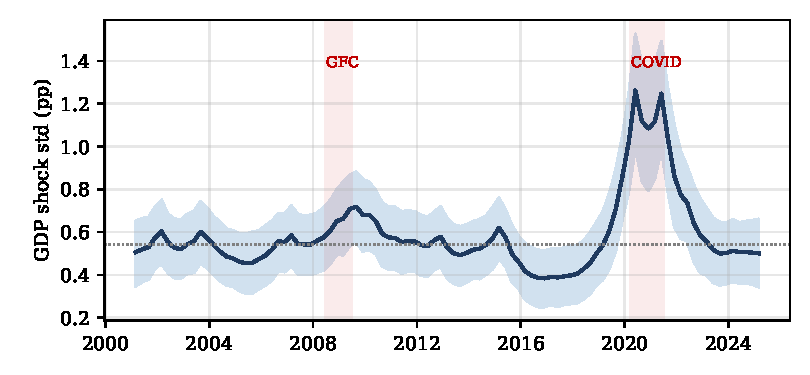
\includegraphics[width=\columnwidth]{fig_sv.pdf}
\caption{Time-varying volatility of GDP-growth shocks from the univariate SV
model (posterior mean and $68\%$ band). Shaded regions mark the Global Financial
Crisis and COVID-19.}
\label{fig:sv}
\end{figure}

\section{Generalization: A G7 Panel}
The preceding analysis is a single-country case study. To establish which findings
are systematic, we replicate the evaluation across five G7 economies---the United
States, United Kingdom, Canada, Germany, and Japan---using comparable quarterly
series from the OECD and Bank for International Settlements (real GDP growth, CPI
inflation, the real effective exchange rate, the 10-year government yield, and a
short/policy rate). Two design choices keep the panel clean. First, the exogenous
block is a \emph{single globally identified shock}---the oil-price surprise---which
is genuinely exogenous to each economy and was the most useful shock in the U.S.\
analysis; this avoids reconstructing nationally specific surrogate shocks of
questionable exogeneity. Second, each economy is run through the \emph{identical}
pipeline, and results are aggregated by pooling one-step loss differentials across
countries for panel Diebold--Mariano tests and by computing a Hansen Model
Confidence Set (MCS) \cite{hansen2011} per variable via a stationary bootstrap.
Samples are 2000--2025 for all economies except Japan (2002--2021, owing to source
data limits), and heterogeneity across countries is treated as a feature.

\begin{table}[t]
\caption{Panel win counts: number of the five economies in which the BVAR achieves
lower one-step CRPS than each benchmark.}
\label{tab:panelwin}
\centering
\footnotesize
\setlength{\tabcolsep}{4pt}
\begin{tabular}{@{}lcccc@{}}
\toprule
Variable & vs.\ RW & vs.\ AR(1) & vs.\ VAR(OLS) & vs.\ no-shock \\
\midrule
GDP growth   & \textbf{5/5} & 3/5 & \textbf{5/5} & 1/5 \\
Inflation    & 3/5 & \textbf{5/5} & \textbf{5/5} & 1/5 \\
REER         & 4/5 & 3/5 & \textbf{5/5} & 4/5 \\
10y yield    & 1/5 & 4/5 & \textbf{5/5} & 2/5 \\
Policy rate  & 4/5 & \textbf{5/5} & \textbf{5/5} & 3/5 \\
\bottomrule
\end{tabular}
\end{table}

Table~\ref{tab:panelwin} reports, for each variable, the number of economies in
which the BVAR attains lower one-step CRPS than each benchmark. The pattern is
consistent with the U.S.\ results and sharper. Shrinkage dominates universally:
the BVAR beats the unrestricted VAR in all five economies for every variable. The
BVAR beats the random walk for output growth everywhere and the no-change forecast
is hardest to beat for the long rate. Against AR(1) the BVAR wins systematically
for inflation and the policy rate. Crucially, the full BVAR rarely beats the
no-shock BVAR (e.g., 1/5 for both GDP and inflation), confirming across countries
that the oil shock does not improve forecasts; the exception is the exchange rate
(4/5), the variable most directly tied to oil.

\begin{table}[t]
\caption{Panel inference: pooled (cross-country) one-step Diebold--Mariano $p$-value
for BVAR vs.\ RW, and the $90\%$ Model Confidence Set among
\{BVAR, no-shock BVAR (nS), VAR(OLS), RW, AR(1)\}.}
\label{tab:panelmcs}
\centering
\footnotesize
\setlength{\tabcolsep}{4pt}
\begin{tabular}{@{}lcl@{}}
\toprule
Variable & Panel DM $p$ (vs.\ RW) & $90\%$ MCS \\
\midrule
GDP growth   & \textbf{0.016} & all five \\
Inflation    & 0.922 & BVAR, nS, RW \\
REER         & 0.292 & BVAR, nS, RW, AR(1) \\
10y yield    & 0.523 & BVAR, nS, RW, AR(1) \\
Policy rate  & \textbf{0.000} & BVAR, nS \\
\bottomrule
\end{tabular}
\end{table}

Pooling loss differentials across countries restores the statistical power that no
single short sample possesses (Table~\ref{tab:panelmcs}). At the panel level the
BVAR significantly outperforms the random walk for output growth ($p=0.016$) and
the policy rate ($p<0.001$); inflation, the exchange rate, and the long yield are
not separable from a no-change forecast. The Model Confidence Set tells a
complementary story: the unrestricted VAR is eliminated for every variable except
GDP, and for the policy rate only the two BVAR variants survive. Fig.~\ref{fig:panel}
displays the underlying heterogeneity---the ratio of BVAR to random-walk CRPS in
each economy---showing that the output-growth advantage holds in all five while the
long-rate disadvantage is similarly broad.

\begin{figure}[t]
\centering
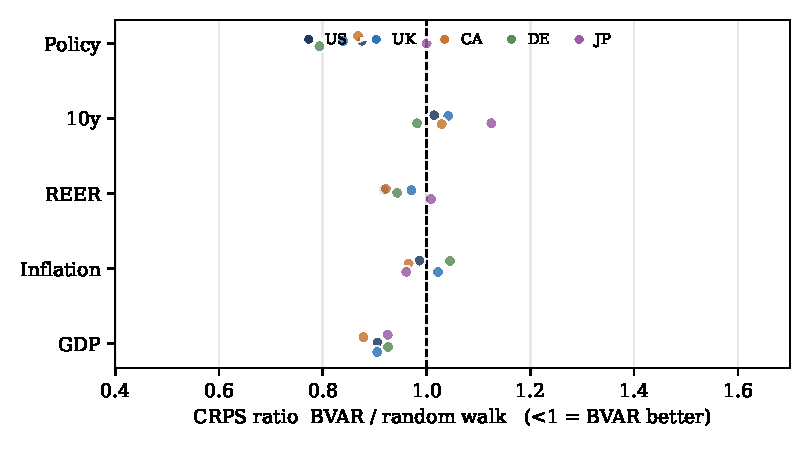
\includegraphics[width=\columnwidth]{fig_panel.pdf}
\caption{One-step CRPS of the BVAR relative to the random walk, by economy and
variable (values below the dashed line indicate the BVAR is better). The
output-growth advantage is systematic across the G7; the long rate is uniformly
hard to beat.}
\label{fig:panel}
\end{figure}

\section{Discussion}
Three lessons generalize beyond this dataset. First, prior \emph{implementation}
matters as much as prior \emph{choice}: a Minnesota prior coded with the wrong
precision/variance convention silently fails to shrink, and dummy observations
are a robust way to avoid this. Second, evaluation design dominates point
estimates. A short window and model-versus-model comparison can manufacture
apparent skill; na\"ive benchmarks, density scoring, and an expanding window are
necessary to separate signal from noise, and on macro data the honest verdict is
often ``competitive but rarely significant.'' Third, diagnostics should precede
machinery: Johansen testing showed that a vector error-correction model was
unnecessary, and a variance diagnostic showed that common stochastic volatility
was the wrong tool, redirecting effort to a variable-specific treatment.

Limitations remain. Although the panel addresses the single-country concern, each
economy still offers only a short quarterly sample ($\sim\!100$ observations or
fewer), which limits the power of forecast comparisons and richly parameterized
volatility models even after cross-country pooling; we use final-vintage rather
than real-time data; the panel relies on a single exogenous shock; and the
country-specific demand-side surrogates in the U.S.\ analysis have questionable
exogeneity. Monthly data and externally identified shocks (high-frequency monetary
surprises, the excess bond premium \cite{gz2012,gss2005}) are natural extensions
that would make per-equation SV and proxy-SVAR identification more credible across
the panel.

\section{Conclusion}
We have presented a transparent, reproducible pipeline for shock-augmented BVAR
forecasting and used it to expose and correct several common failures:
mis-specified Minnesota shrinkage, shock-combination overfitting, the absence of
na\"ive benchmarks and significance testing, look-ahead leakage in shock
construction, and an inappropriate common-volatility assumption. Once these are
addressed, a correctly specified stochastic-volatility BVAR delivers sharper,
better-calibrated density forecasts than random-walk and AR(1) benchmarks for
output growth and inflation, while interest rates remain difficult to beat.
Extending the study to a five-economy G7 panel shows these conclusions are
systematic rather than U.S.-specific: Bayesian shrinkage dominates an unrestricted
VAR in every country, the BVAR significantly beats the random walk for output
growth and the policy rate when evidence is pooled across countries, and the
constructed shocks improve fit but not multi-step forecasts everywhere. The
contribution is less a new model than a disciplined, cross-country protocol for
deciding when a shock-augmented BVAR genuinely adds forecasting value.

\section*{Reproducibility}
All estimation, evaluation, and figure code, together with the corrected BVAR,
leak-free shock construction, the cointegration and identification diagnostics,
the expanding-window density evaluation, and the SV sampler, are provided as
self-contained Python modules.

\begin{thebibliography}{00}
\bibitem{sims1980} C.~A. Sims, ``Macroeconomics and reality,''
\emph{Econometrica}, vol.~48, no.~1, pp.~1--48, 1980.
\bibitem{litterman1986} R.~B. Litterman, ``Forecasting with Bayesian vector
autoregressions---five years of experience,'' \emph{J.\ Bus.\ Econ.\ Stat.},
vol.~4, no.~1, pp.~25--38, 1986.
\bibitem{doan1984} T.~Doan, R.~Litterman, and C.~Sims, ``Forecasting and
conditional projection using realistic prior distributions,'' \emph{Econometric
Rev.}, vol.~3, no.~1, pp.~1--100, 1984.
\bibitem{bgr2010} M.~Ba\'nbura, D.~Giannone, and L.~Reichlin, ``Large Bayesian
vector auto regressions,'' \emph{J.\ Appl.\ Econometrics}, vol.~25, no.~1,
pp.~71--92, 2010.
\bibitem{sims1998} C.~A. Sims and T.~Zha, ``Bayesian methods for dynamic
multivariate models,'' \emph{Int.\ Econ.\ Rev.}, vol.~39, no.~4, pp.~949--968,
1998.
\bibitem{kadiyala1997} K.~R. Kadiyala and S.~Karlsson, ``Numerical methods for
estimation and inference in Bayesian VAR-models,'' \emph{J.\ Appl.\
Econometrics}, vol.~12, no.~2, pp.~99--132, 1997.
\bibitem{koop2010} G.~Koop and D.~Korobilis, ``Bayesian multivariate time series
methods for empirical macroeconomics,'' \emph{Found.\ Trends Econometrics},
vol.~3, no.~4, pp.~267--358, 2010.
\bibitem{giannone2015} D.~Giannone, M.~Lenza, and G.~E. Primiceri, ``Prior
selection for vector autoregressions,'' \emph{Rev.\ Econ.\ Stat.}, vol.~97,
no.~2, pp.~436--451, 2015.
\bibitem{dm1995} F.~X. Diebold and R.~S. Mariano, ``Comparing predictive
accuracy,'' \emph{J.\ Bus.\ Econ.\ Stat.}, vol.~13, no.~3, pp.~253--263, 1995.
\bibitem{hln1997} D.~Harvey, S.~Leybourne, and P.~Newbold, ``Testing the
equality of prediction mean squared errors,'' \emph{Int.\ J.\ Forecasting},
vol.~13, no.~2, pp.~281--291, 1997.
\bibitem{gneiting2007} T.~Gneiting and A.~E. Raftery, ``Strictly proper scoring
rules, prediction, and estimation,'' \emph{J.\ Amer.\ Statist.\ Assoc.},
vol.~102, no.~477, pp.~359--378, 2007.
\bibitem{jorda2005} \`O.~Jord\`a, ``Estimation and inference of impulse responses
by local projections,'' \emph{Amer.\ Econ.\ Rev.}, vol.~95, no.~1, pp.~161--182,
2005.
\bibitem{johansen1991} S.~Johansen, ``Estimation and hypothesis testing of
cointegration vectors in Gaussian vector autoregressive models,''
\emph{Econometrica}, vol.~59, no.~6, pp.~1551--1580, 1991.
\bibitem{primiceri2005} G.~E. Primiceri, ``Time varying structural vector
autoregressions and monetary policy,'' \emph{Rev.\ Econ.\ Stud.}, vol.~72, no.~3,
pp.~821--852, 2005.
\bibitem{ksc1998} S.~Kim, N.~Shephard, and S.~Chib, ``Stochastic volatility:
likelihood inference and comparison with ARCH models,'' \emph{Rev.\ Econ.\
Stud.}, vol.~65, no.~3, pp.~361--393, 1998.
\bibitem{ccm2016} A.~Carriero, T.~E. Clark, and M.~Marcellino, ``Common drifting
volatility in large Bayesian VARs,'' \emph{J.\ Bus.\ Econ.\ Stat.}, vol.~34,
no.~3, pp.~375--390, 2016.
\bibitem{clark2011} T.~E. Clark, ``Real-time density forecasts from Bayesian
vector autoregressions with stochastic volatility,'' \emph{J.\ Bus.\ Econ.\
Stat.}, vol.~29, no.~3, pp.~327--341, 2011.
\bibitem{kilian2009} L.~Kilian, ``Not all oil price shocks are alike:
disentangling demand and supply shocks in the crude oil market,'' \emph{Amer.\
Econ.\ Rev.}, vol.~99, no.~3, pp.~1053--1069, 2009.
\bibitem{gz2012} S.~Gilchrist and E.~Zakraj\v{s}ek, ``Credit spreads and business
cycle fluctuations,'' \emph{Amer.\ Econ.\ Rev.}, vol.~102, no.~4,
pp.~1692--1720, 2012.
\bibitem{gss2005} R.~S. G\"urkaynak, B.~Sack, and E.~T. Swanson, ``Do actions
speak louder than words? The response of asset prices to monetary policy actions
and statements,'' \emph{Int.\ J.\ Central Banking}, vol.~1, no.~1, pp.~55--93,
2005.
\bibitem{stockwatson2012} J.~H. Stock and M.~W. Watson, ``Disentangling the
channels of the 2007--09 recession,'' \emph{Brookings Papers Econ.\ Activity},
pp.~81--135, Spring 2012.
\bibitem{mertensravn2013} K.~Mertens and M.~O. Ravn, ``The dynamic effects of
personal and corporate income tax changes in the United States,'' \emph{Amer.\
Econ.\ Rev.}, vol.~103, no.~4, pp.~1212--1247, 2013.
\bibitem{lenza2022} M.~Lenza and G.~E. Primiceri, ``How to estimate a vector
autoregression after March 2020,'' \emph{J.\ Appl.\ Econometrics}, vol.~37,
no.~4, pp.~688--699, 2022.
\bibitem{carter1994} C.~K. Carter and R.~Kohn, ``On Gibbs sampling for state
space models,'' \emph{Biometrika}, vol.~81, no.~3, pp.~541--553, 1994.
\bibitem{hansen2011} P.~R. Hansen, A.~Lunde, and J.~M. Nason, ``The model
confidence set,'' \emph{Econometrica}, vol.~79, no.~2, pp.~453--497, 2011.
\end{thebibliography}

\end{document}
